\chapter{Entropy and Its Interpretations}

Consider a random variable \( X \) taking values in an alphabet \( \mathcal{X} = \{x_1, \dots, x_l\} \).

\defb{Definition: Information Content}{
    The \textit{information content} (also known as surprise or surprisal) of a realisation \( x \) is defined as:
    \[
        h(x) := \log \frac{1}{p(x)}
    \]
}

\defb{Definition: Entropy}{
    The \textit{entropy} of a random variable \( X \) is given by:
    \[
        H(X) := \sum_{x \in \mathcal{X}} p(x) \log \frac{1}{p(x)}
    \]
    Entropy represents the expected value of the information content (or surprisal) across all possible realisations of \( X \):
    \[
        H(X) = \mathbb{E}[h(X)] = \sum_x p(x) h(x)
    \]
}

\section{Entropy of a Biased Coin}

Let $X$ be a coin flip from a biased coin with alphabet $\mathcal{X} = \{H, T\}$ and probabilities $(p, 1-p)$. The entropy of $X$ is given by the binary entropy function:

\marginnote[-10pt]{This is the expected value of surprisal when flipping a biased coin. }

\[
    H(p) = -p \log p - (1-p) \log (1-p)
\]

\begin{figure*}[h]
    \centering
    \begin{minipage}{0.3\textwidth}
        \centering
        % Plot h(p) = log2(1/p)
        \begin{tikzpicture}
            \begin{axis}[
                    domain=0.001:1,
                    samples=100,
                    width=\textwidth,
                    height=0.8\textwidth,
                    xlabel={$p$},
                    ylabel={$h(p)$},
                    ytick={0,2,4,6,8,10},
                    ymin=0, ymax=10,
                    xmin=0, xmax=1,
                    axis lines=left,
                    every axis y label/.style={at={(current axis.above origin)},anchor=south},
                    every axis x label/.style={at={(current axis.right of origin)},anchor=west}
                ]
                \addplot[black, thick] {log2(1/x)};
                \node[above right] at (axis cs:0.3,7) {$h(p) = \log_2 \frac{1}{p}$};
            \end{axis}
        \end{tikzpicture}
    \end{minipage}
    \hfill
    \begin{minipage}{0.3\textwidth}
        \centering
        % Table for values of p, h(p), and H2(p)
        \renewcommand{\arraystretch}{1.2}
        \begin{tabular}{ccc}
            \hline
            $p$   & $h(p)$ & $H_2(p)$ \\
            \hline
            0.001 & 10.0   & 0.011    \\
            0.01  & 6.6    & 0.081    \\
            0.1   & 3.3    & 0.47     \\
            0.2   & 2.3    & 0.72     \\
            0.5   & 1.0    & 1.0      \\
            \hline
        \end{tabular}
    \end{minipage}
    \hfill
    \begin{minipage}{0.3\textwidth}
        \centering
        % Plot H2(p) = -p*log2(p) - (1-p)*log2(1-p)
        \begin{tikzpicture}
            \begin{axis}[
                    domain=0.001:1,
                    samples=100,
                    width=\textwidth,
                    height=0.8\textwidth,
                    xlabel={$p$},
                    ylabel={$H_2(p)$},
                    ymin=0, ymax=1,
                    xmin=0, xmax=1,
                    axis lines=left,
                    every axis y label/.style={at={(current axis.above origin)},anchor=south},
                    every axis x label/.style={at={(current axis.right of origin)},anchor=west}
                ]
                \addplot[black, thick] {-x*log2(x) - (1-x)*log2(1-x)};
                \node[above] at (axis cs:0.5,0.5) {$H_2(p)$};
            \end{axis}
        \end{tikzpicture}
    \end{minipage}
    \vspace{10pt}
    \caption{Unlikely outcomes provide more information – but if the outcomes of the coin are skewed towards one side, the overall entropy decreases, because the extra information gained by the rarer outcome is diminished by the expectation, where it doesn't happen often enough, reducing the total expected surprise.}
    \label{fig:entropy_coin}
\end{figure*}

Matehmatically, a biased coin flip $X$ is just the \textbf{Bernoulli distribution} with parameter $p$:
\[
    X \sim \mc{B}(p)
\]

\sn{The units of \ensuremath{h(x)}}{
    The units of $h(x)$ depend on the base of the log– $\log_2$ is for bits, $\log_{10}$ is for dits, and $\log_e$ is for nats.
}

\defb{Terminology of `Bit'}{
    We denote two things with \textbf{bit}:
    \begin{enumerate}
        \item The units of information content, taken with $\log_2$.
        \item A random variable with alphabet $\{0, 1\}$.
    \end{enumerate}
}

\section{Properties of Entropy in Discrete Distributions}

\begin{itemize}
    \item The entropy of discrete distributions is non-negative.
    \item The general bound on discrete entropy is \( 0 \leq H(X) \leq \log |\mathcal{X}| \).
    \item Entropy is minimised for the Kronecker delta distribution, (i.e. $p_i = 1, p_{j \neq i} = 0$). For example, take the Kronecker delta function \(\delta_{i3}\):
          \[
              \delta_{i3} = \begin{cases}
                  1 & \text{if } i = 3 \\
                  0 & \text{otherwise}
              \end{cases}
          \]
          \begin{center}
              \begin{tikzpicture}
                  % Set up the axis
                  \draw[->] (-0.5,0) -- (6.5,0) node[right] {$i$};  % x-axis
                  \draw[->] (0,-0) -- (0,1.5) node[above] {$\delta_{i3}$}; % y-axis

                  % Label x-axis values
                  \foreach \x in {0, 1, 2, 3, 4, 5, 6}
                  \draw (\x,0) -- (\x,-0.1) node[below] {\x};

                  % Draw Kronecker delta "spikes"
                  \foreach \x in {0, 1, 2, 4, 5, 6}
                  \draw[thick] (\x, 0) -- (\x, 0); % Zero-height "bars"

                  % Draw the "spike" at i = 3
                  \filldraw[blue] (3,0) rectangle (3.04,1);  % Bar at i = 3
                  \node[above, blue] at (3,1) {1};  % Label the height of the delta function

                  % Label for Kronecker delta
                  \node[right] at (3.2, 1) {\(\delta_{i3}\)};
              \end{tikzpicture}
          \end{center}
          Calculating entropy for this distribution:
          \[
              H(X) = \left( 1 \cdot \log 1 + \sum_{i \neq 3} 0 \cdot \log 0 \right) = 0
          \]

    \item Entropy is maximised for the uniform distribution
\end{itemize}

\intuitb{Impossible Events– What if \ensuremath{p_j = 0}?}{
    The mathematical convention is to treat $0 \log 0 = 0$ – impossible events do not change entropy.
}


\section{Independent Random Variables}

What happens if I flip two coins separately? Consider two independent flips $X$ and $Y$. Recall for independent RVs, $P(X, Y) = P(X)P(Y)$. The joint entropy of $X$ and $Y$ is given by:

\begin{align*}
    h(x, y) &= -\log P(x, y) \\
            &= -\log \big(P(x) P(y)\big) \\
            &= -\log P(x) - \log P(y) \\
            &= h(x) + h(y)
\end{align*}

Similarly for entropy, note that \textbf{entropy is additive for independent random variables:}


\begin{align*}
    H(X, Y) &= \sum_{\textcolor{blue}{x}, \textcolor{red}{y}} P(x, y) h(x, y) \\
            &= \sum_{\textcolor{blue}{x}, \textcolor{red}{y}} \textcolor{blue}{P(x)} \textcolor{red}{P(y)} h(x, y) + \sum_{\textcolor{blue}{x}, \textcolor{red}{y}} P(x) P(y) h(y) \\
            &= \textcolor{red}{\cancel{\underbrace{\sum_{y} \textcolor{red}{P(y)}}_{\textcolor{red}{1}}}} 
               \cdot \textcolor{blue}{\sum_{x} \textcolor{blue}{P(x)} h(x)} 
               + \cancel{\underbrace{\sum_{x} P(x)}_{1}} \cdot \sum_{y} P(y) h(y) \\
            &= \textcolor{blue}{H(X)} + H(Y).
\end{align*}

\defb{Shannon Axioms}{
The surprisal of an event with probability \( p \), \( i(p) \) must satisfy:
\begin{enumerate}
    \item Certain events are unsurprising: \( i(1) = 0 \).
    \item Less probable events are more surprising: \( \frac{di}{dp} \leq 0 \).
    \item Independent events yield the sum of their surprisals:
    \[
        i(p \cdot q) = i(p) + i(q).
    \]
\end{enumerate}
The only function satisfying these axioms is the negative logarithm:
\[
    i(p) = h(p) = -\log_b(p)
\]

\textit{Note: There are many equivalent sets of axioms for entropy.}
}

\section{Information Gain}

\subsection{A Number Guessing Game}

In the game \textit{Who's Who}, one player picks a character, and the other asks yes-or-no questions to guess their identity, such as:
\begin{itemize}
    \item Are they wearing glasses?
    \item Do they have a moustache?
\end{itemize}

To explore a simpler variation, consider a game called \textit{Sixty-Three}:
\begin{itemize}
    \item One player selects an integer \( x \) from 0 to 63.
    \item The other player asks questions to guess \( x \).
\end{itemize}

\textbf{Optimal Questions:} One possible set of optimal questions:
\begin{enumerate}
    \item Is \( x \geq 32 \)?
    \item Is \( x \mod 32 \geq 16 \)?
    \item \dots
    \item Is \( x \mod 2 = 1 \)?
\end{enumerate}

This strategy defines a map \( \{0, \dots, 63\} \to \{0,1\}^6 \), where each output bit is the answer to a specific question. For example, \( x = 35 \) corresponds to \( 100011 \).

If \( x \) is uniformly distributed, each answer provides 1 bit of information, calculated as \( h = -\log(1/2) = 1 \) bit. Thus, the total information gained is 6 bits.

Information content corresponds to the length of the binary encoding of \( x \).

\subsection{A Submarine Guessing Game}

\begin{itemize}
    \item I pick one of 64 squares to hide a submarine.
    \item In each round, you fire at one square, resulting in a ‘hit’ or ‘miss.’
\end{itemize}

(The difference with \textit{sixty-three} is that you always fire to just one square.)

\begin{figure*}
    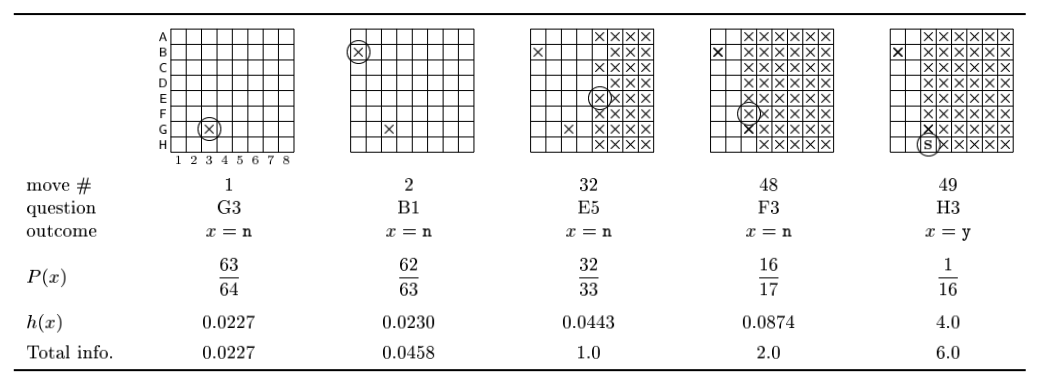
\includegraphics[width=0.9\linewidth]{img/submarines.png}
\end{figure*}

\begin{itemize}
    \item \textbf{Scenario 1:} You hit the submarine with the first question.
    \begin{itemize}
        \item You obtain \( \log(64) = 6 \) bit.
    \end{itemize}

    \item \textbf{Scenario 2:} You miss 32 times, then hit.
    \begin{itemize}
        \item The first miss gives you \( \log(64/63) = 0.0227 \) bit.
        \item By the 32\textsuperscript{nd} miss, you have
        \[
            \log(64/63) + \log(63/62) + \dots + \log(33/32) = 0.0227 + 0.0230 + \dots + 0.0444 = 1 \text{ bit}.
        \]
        \item The hit gives you \( \log(32) = 5 \) bit, for a total of 6 bit.
    \end{itemize}

    \item \textbf{General case:} You miss \( 64 - n \), then hit:
    \[
        \underbrace{\log \frac{64}{63} + \log \frac{63}{62} + \dots + \log \frac{n+1}{n}}_{\text{misses}} + \underbrace{\log \frac{n}{1}}_{\text{hit}} = \log 64 = 6 \text{ bit}
    \]

    \item \textbf{Conclusion:} Regardless of when you hit, you always get 6 bit.
\end{itemize}

\intuitb{Conclusions}{
\begin{itemize}
    \item For uniform distributions, \( h(x) \) corresponds to the length of the \textbf{binary representation} of \( x \) (i.e., number of yes/no questions).
    
    \item \( h(x) \) is a measure of the \textbf{“intrinsic”} information content of \( x \), regardless of how that information is obtained.
    
    \item Information is given by \textbf{probability mass exclusions} (Hartley 1928).
\end{itemize}

The goal of experiments is to \textbf{reduce uncertainty} about something by excluding possibilities. The takeaway is that you should design experiemtns with evenly probable outcomes to maximise information gain, as shown in Figure \ref{fig:entropy_coin}.
}

\section{Entropy in Continuous Distributions}

We have explored entropy in discrete RVs with finite alphabets, we then extend this to continuous RVs– by discretising the variable's continous domain.

\begin{itemize}
    \item We have a random variable \( X \in \mathbb{R} \) with PDF \( f(x) \).
    \item We use bins of width \( \Delta \) to get a discrete variable \( X^{\Delta} \) with
    \[
        p_i = \int_{(i - \frac{1}{2})\Delta}^{(i + \frac{1}{2})\Delta} f(x) \, dx = f(x_i) \Delta
    \]
    \item Now we take \( H(X^{\Delta}) \) as \( \Delta \to 0 \):
    \begin{align*}
        H(X^{\Delta}) &= -\sum p_i \log p_i \\
        &= -\sum f(x_i) \Delta \log(f(x_i) \Delta) \\
        &= -\sum \Delta f(x_i) \log f(x_i) - \log \Delta \\
        &= \underbrace{-\sum \Delta f(x_i) \log f(x_i)}_{\text{Riemann integral}}  \underbrace{- \log \Delta}_{\text{Divergent term}}
    \end{align*}
    \item Oh no, \( \lim_{\Delta \to 0} \log \Delta = -\infty \), so \( H(X^{\Delta}) \) diverges for any \( f(x) \).
    \item A foolproof strategy is to ignore $\log \Delta$ anyway, and define the \textbf{differential entropy} as:
\end{itemize}

\defb{Definition: Differential entropy}{
The \textit{differential entropy} of a continuous RV \( X \) with PDF \( f(x) \) is given by
\[
    H(X) := - \int f(x) \log f(x) \, dx
\]
}

\sn{Warning}{
The \( \log \Delta \) will come back to haunt us! Differential entropy lacks many interesting properties of discrete entropy. \bigskip 

\textbf{Disclaimer:} We may use the term ‘entropy’ for continuous RVs too.
}

\subsection{Properties of Differential Entropy}
Take an example of differential entropy in uniform distributions:
Let \( X \) be a uniform random variable in the interval of length \( a \).

\[
X \sim \mathcal{U}([0, a]) \quad \text{i.e.} \quad p(x) = \frac{1}{a}
\]

\[
H(X) = - \int_0^a \frac{1}{a} \log \frac{1}{a} \, dx = - \log \frac{1}{a} \int_0^a \frac{dx}{a} = \log a
\]

\textbf{Conclusions:} We see that Differential entropy:
\begin{itemize}
    \item Can be negative, e.g. for $a < 1$.
    \item Grows with the volume of the distribution $(2^{H(X)} = a > 0)$
\end{itemize}

\subsection{Surprisal in Gaussian Distributions}

\marginnote{\intuitsb{Modelling \ensuremath{x}}{We want to reduce surprisal to ensure we can compactly encode $x$ more efficiently. In this example, we want to model \( x \) with the Gaussian distribution. Reducing surprisal is then equivalent to reducing the prediction error, or the mean squared error (MSE). \bigskip

Try to imagine a distribution of $x$ and then we play around with the parameters of a Gaussian distribution to make it fit the distribution of $x$ better. \bigskip

If we find a more accurate $\mu$ for our model, we then reduce the MSE. And if our $\mu$ is already quite close to the true value of $x$, increasing precision (making reducing $\sigma$ to make the distribution more narrow, centring closer around $\mu$) can also sometimes reduce surprisal. However, if $\mu$ is too far from the true value of $x$, increasing precision can sometimes increase surprisal.}}

Let \( X \sim \mathcal{N}(\mu, \sigma^2) \) be a 1D Gaussian random variable, i.e.
\[
p(x) = \left( \sigma \sqrt{2 \pi} \right)^{-1} e^{-\frac{1}{2} \left( \frac{x - \mu}{\sigma} \right)^2}
\]


Then, surprisal is just the negative $ln$ of the PDF:
\[
h(x) = \ln \left( \sigma \sqrt{2 \pi} \right) + \frac{1}{2} \left( \frac{x - \mu}{\sigma} \right)^2
\]

This expression is equivalent to scaled mean squared error (MSE):
\[
h(x) = \ln \sigma + \frac{1}{2 \sigma^2} \text{MSE}(x, \mu) + C.
\]

If we predict \( x \) with a PDF \( \mathcal{N}(\mu, \sigma^2) \), we can lower the surprisal by:

\begin{itemize}
    \item Reducing the bias (i.e., moving \( \mu \) closer to \( x \)),
    \item (Sometimes) increasing the precision (i.e., increasing \( \sigma \)).
\end{itemize}


\subsection{Entropy in Gaussian Distributions}

We show that Entropy has a closed-form expression for Gaussian Distributions:

To calculate the entropy of a \(D\)-dimensional Gaussian distribution \(\mathcal{N}(\mu, \Sigma)\),

\[
p(x) = |2 \pi \Sigma|^{-1/2} \exp \left( -\frac{1}{2} (x - \mu)^\top \Sigma^{-1} (x - \mu) \right).
\]

The entropy \(H(X)\) is given by:
\[
H(X) = - \int_{-\infty}^{+\infty} \mathcal{N}(x; \mu, \Sigma) \ln \mathcal{N}(x; \mu, \Sigma) \, dx.
\]

Expanding, we get:
\[
H(X) = \frac{1}{2} \mathbb{E}[\ln |2 \pi \Sigma|] + \frac{1}{2} \mathbb{E}[(x - \mu)^\top \Sigma^{-1} (x - \mu)].
\]

For the first term, \(\mathbb{E}[\ln |2 \pi \Sigma|] = \ln |2 \pi \Sigma|\).

For the second term:
\[
\mathbb{E} \left[ (x - \mu)^\top \Sigma^{-1} (x - \mu) \right] = \operatorname{tr} \left( \Sigma^{-1} \mathbb{E} \left[ (x - \mu)(x - \mu)^\top \right] \right) = \operatorname{tr}(\Sigma^{-1} \Sigma) = D.
\]

Substituting back, we get:
\[
H(X) = \frac{1}{2} \ln |2 \pi \Sigma| + \frac{1}{2} D = \frac{1}{2} \ln \left( |2 \pi \Sigma| e^D \right).
\]

Overall:
\[
H(X) = \frac{1}{2} \ln |2 \pi e \Sigma|.
\]

\subsection{Takeaways of Entropy}
\begin{itemize}
    \item Entropy quantifies the \textbf{average information content} of an observation \(x\).
    \item Entropy serves as a \textbf{generalised variance} (e.g., measures predictability of \(X\)).
    \item For discrete distributions:
    \begin{itemize}
        \item Entropy is \textbf{bounded}: \(0 \leq H(X) \leq \log |\mathcal{X}|\).
        \item Related to the \textbf{number of yes/no questions} needed to determine \(x\).
    \end{itemize}
    \item For continuous distributions, \textbf{differential entropy} is defined, but can be negative and lacks some properties of discrete entropy.
\end{itemize}

\section{Source Coding Theorem}

\defb{Definition: Code and Code Length}{
    Given a random variable \( X \) with alphabet \( \mathcal{X} \) and an alphabet \( \mathcal{D} \), a \textbf{code} is a mapping
    \[
        C : \mathcal{X} \to \mathcal{D}^*,
    \]
    where \( \mathcal{D}^* \) is the set of all finite-length strings of symbols in \( \mathcal{D} \).

    The quantity \( \ell(x) \) is the \textbf{code length} of \( C(x) \), and \( L = \mathbb{E}[\ell(x)] \) the \textbf{average code length}.
}

\begin{itemize}
    \item For each symbol \( x \), the string \( C(x) \in \mathcal{D}^* \) is called a \textbf{codeword}.
    \item When \( |\mathcal{D}| = 2 \), \( C \) is a \textbf{binary code}. When \( |\mathcal{D}| = d \), \( C \) is a \textbf{d-ary code}.
\end{itemize}

Here are two example codes for the alphabet \( \mathcal{X} = \{ \text{a}, \text{b}, \text{c}, \text{d} \} \).

\begin{table}[h]
    \centering
    \begin{tabular}{c@{\hskip 1cm}c}
        \begin{tabular}{cc}
            \toprule
            \multicolumn{2}{c}{Binary} \\
            \midrule
            \( x \) & \( C(x) \) \\
            \midrule
            a & 00 \\
            b & 01 \\
            c & 10 \\
            d & 11 \\
            \bottomrule
        \end{tabular}
        &
        \begin{tabular}{cc}
            \toprule
            \multicolumn{2}{c}{Ternary} \\
            \midrule
            \( x \) & \( C(x) \) \\
            \midrule
            a & 0 \\
            b & 1 \\
            c & 2 \\
            d & 200 \\
            \bottomrule
        \end{tabular}
    \end{tabular}
\end{table}


\subsection{Coding for the Uniform Distribution}

\begin{itemize}
    \item We’ve seen that (in uniform distributions), entropy corresponds to the number of \textbf{yes/no} questions needed to guess \( x \).
    
    \[
    \begin{array}{c@{\quad\Rightarrow\quad}c@{\quad}c@{\quad\Rightarrow\quad}c}
        35 & 100011 & 6 & 000110 \\
        0 & 000000 & 17 & 010001 \\
        42 & 101010 & \dots & \dots \\
    \end{array}
    \]

    \item This forms a \textbf{binary code} for \( X \) with length
    \[
        L = H(X) = \log |\mathcal{X}|.
    \]

    \item More generally, \( \log |\mathcal{X}| \) is referred to as the \textbf{raw bit content} of \( X \).
\end{itemize}

\sn{Warning: Ceiling and the “Extra Bit”}{
    When \( |\mathcal{X}| \) is not a power of two, we may need an “extra bit” to encode symbols. You may see this written as \( L = \lceil \log |\mathcal{X}| \rceil \) or \( L = \log |\mathcal{X}| + 1 \).
}


\subsection{Non-uniform Distributions}

What happens when the distribution isn’t uniform?



\begin{itemize}
    \item \textbf{Example}: compressing Wikipedia, which has alphabet \( \mathcal{X} = \mathcal{E} \cup \mathcal{U} \):
    \begin{itemize}
        \item \( \mathcal{E} \) is the English alphabet, \( |\mathcal{E}| = 26 \);
        \item \( \mathcal{U} = \{ !, @, \#, \$, \%, -, \&, *, (, ) \} \) includes some unicode characters.
    \end{itemize}

    \item Assume that 98\% of Wikipedia content comes from \( \mathcal{E} \), and 2\% from \( \mathcal{U} \).

    \item A naive binary code of \( \mathcal{X} \) would require \( \lceil \log |\mathcal{X}| \rceil = \lceil \log 36 \rceil = 6 \) bits.

    \item \textbf{But}... if we ignore \( \mathcal{U} \), we can encode in \( \lceil \log |\mathcal{E}| \rceil = \lceil \log 26 \rceil = 5 \) bits.
\end{itemize}

\sn{Reduction in Code Length}{
    We have \textbf{reduced the code length} with only \textbf{2\% error}, simply by refusing to encode the minority of rarely-used symbols. And this generally would not have a major impact on the readability of the text– most information could still be conveyed.
}


\subsection{Law of Large Numbers}

The Law of Large Numbers states that as the number of independent, identically distributed (i.i.d.) random variables increases, their sample average converges to the expected value. This result forms a cornerstone of probability and statistics, establishing that with a large enough sample size, we can expect the sample mean to approximate the population mean closely.

\begin{itemize}
    \item Let \( Y^n = \frac{1}{n} \sum_{i=1}^n X_i \) be the mean of \(n\) i.i.d. random variables \( X_1, \dots, X_n \), with
    \[
    \mathbb{E}[X_1] = \dots = \mathbb{E}[X_n] = \mu \quad \text{and} \quad \operatorname{Var}(X_i) = \dots = \operatorname{Var}(X_n) = \sigma^2.
    \]

    \item By direct calculation, it can be shown that:
    \[
    \mathbb{E}[Y^n] = \mu \quad \text{and} \quad \operatorname{Var}(Y^n) = \frac{\sigma^2}{n}.
    \]

    \item As \( n \to \infty \), \( Y^n \) has \textbf{vanishing variance}, meaning \( Y^n \) becomes increasingly close to \( \mu \).
\end{itemize}

\thm{Weak Law of Large Numbers}{
    Let \( Y^n = \frac{1}{n} \sum_{i=1}^n X_i \). As \( n \to \infty \), \( Y^n \) converges in probability to \( \mu \):
    \[
    Y^n \xrightarrow{P} \mu, \quad \text{that is,} \quad \lim_{n \to \infty} \Pr\left( |Y^n - \mu| < \varepsilon \right) = 1
    \]
    for any \( \varepsilon > 0 \).
}
